% This is samplepaper.tex, a sample chapter demonstrating the
% LLNCS macro package for Springer Computer Science proceedings;
% Version 2.20 of 2017/10/04
%
\documentclass[runningheads]{llncs2e/llncs}
%
\usepackage{graphicx}
\usepackage{xspace}
\usepackage[dvipsnames]{xcolor}
\usepackage{amsmath}
\usepackage{afterpage}  
\usepackage{figlatex,wrapfig}
\usepackage[dvipsnames]{xcolor}
\usepackage{listings,amssymb,mathtools}
\usepackage{mathrsfs}
\usepackage{array,multirow}
\usepackage{caption}
%\usepackage{textcomp}
\usepackage{algorithm}
\usepackage[noend]{algpseudocode}
\usepackage{framed,enumitem}

% for colours
\usepackage{xspace}
\usepackage[colorlinks]{hyperref}
\hypersetup{
	colorlinks = true,
	citecolor = {violet},
	linkcolor = {blue},
	urlcolor  = {blue}
}

% for arrow diagrams
\usepackage{amsmath}
\usepackage{amssymb}
\usepackage{smartdiagram}
\usepackage{tikz}
\usetikzlibrary{arrows,positioning}

%\usepackage[parfill]{parskip}

% for bib handline
%\usepackage[numbers]{natbib}
%\usepackage{url}

% implies and iff arrows
\renewcommand{\iff}{\xspace\Leftrightarrow\xspace}
\renewcommand{\implies}{\xspace\Rightarrow\xspace}
\newcommand{\onlyif}{\xspace\Leftarrow\xspace}

% commonly used abbreviations and expressions
\renewcommand{\th}{^{th}\xspace} % superscript th for numbers eg i^{th}
\newcommand{\definedas}{\triangleq\xspace}
\newcommand{\ie}{{\em i.e.}\xspace}
\newcommand{\st}{\ \mbox{s.t.}\ }
\newcommand{\viz}{\textit{viz}.\@\xspace}
\newcommand{\wrt}{\textit{wrt}\xspace}
\newcommand{\wkt}{we know that,\xspace}
\newcommand{\aka}{a.k.a\xspace}
\newcommand{\sota}{state-of-the-art\xspace}
\newcommand{\Sota}{State-of-the-art\xspace}

% common operators
\renewcommand{\^}{\xspace\wedge\xspace}
\renewcommand{\v}{\xspace\vee\xspace}
\newcommand{\xor}{\xspace\veebar\xspace}
\renewcommand{\|}{\ |\ }
\newcommand{\intersection}{\xspace\cap\xspace}
\newcommand{\union}{\xspace\cup\xspace}
\newcommand{\intersectioneq}{\xspace\cap=\xspace}
\newcommand{\unioneq}{\ {\cup}{=}\ }
\newcommand{\nin}{\not\in\xspace}

% highlighted hyperlinks
\newcommand{\hl}[1]{{\textcolor{darkgray}{\texttt{(#1)}}}\xspace} % hyperlink target
\newcommand{\hlref}[1]{\hyperlink{#1}{\textcolor{Sepia}{\small \texttt{(#1)}}}}
\newcommand{\tab}{\quad\quad}

%%%%%%%%%%%%%%%%%%%%%%%%% Document Specific %%%%%%%%%%%%%%%%%%%%%%

% names
\newcommand{\ourtechnique}{\textcolor{RubineRed}{\texttt{FenSyn}}\xspace}
\newcommand{\ourtool}{\ourtechnique{-}tool\xspace}
\newcommand{\cc}{\textit{C11}\xspace}

% sets and entitites
\newcommand{\program}{$P$\xspace} %input program
\newcommand{\programhat}{$\widehat{P}$\xspace} %transformed/fixed program
\newcommand{\fixed}[1]{\widehat{#1}\xspace}
\newcommand{\threads}{\mathcal{T}\xspace}
\newcommand{\states}{\Sigma\xspace}
\newcommand{\moset}{\mathcal{M}\xspace}
\newcommand{\actions}{\mathcal{A}\xspace}
\newcommand{\objects}{\mathcal{O}\xspace}
\newcommand{\s}[1]{s_{[#1]}\xspace} % state reached after exploring sequence #1
% events' sets aux
\newcommand{\wt}[1]{{\mathbb{W}#1}}
\newcommand{\md}[1]{{\mathbb{M}#1}}
\newcommand{\rd}[1]{{\mathbb{R}#1}}
\newcommand{\fn}[1]{{\mathbb{F}#1}}
% events' sets
\newcommand{\events}{\mathcal{E}\xspace}
\newcommand{\writes}{\events^\wt{}\xspace}
\newcommand{\reads}{\events^\rd{}\xspace}
\newcommand{\fences}{\events^\fn{}\xspace}
\newcommand{\ordevents}[1]{\events^{(#1)}\xspace}
\newcommand{\ordwrites}[1]{\events^\wt{(#1)}\xspace}
\newcommand{\ordreads}[1]{\events^\rd{(#1)}\xspace}
\newcommand{\ordfences}[1]{\events^\fn{(#1)}\xspace}


% memory orders
\newcommand{\mosc}{\texttt{seq\_cst}\xspace}
\newcommand{\moar}{\texttt{acq\_rel}\xspace}
\newcommand{\morel}{\texttt{release}\xspace}
\newcommand{\moacq}{\texttt{acquire}\xspace}
\newcommand{\mocon}{\texttt{consume}\xspace}
\newcommand{\morlx}{\texttt{relaxed}\xspace}

% operators
\newcommand{\molt}{{\sqsubset}\xspace}
\newcommand{\mole}{{\sqsubseteq}\xspace}
\newcommand{\mogt}{{\sqsupset}\xspace}
\newcommand{\moge}{{\sqsupseteq}\xspace}

% relations
\newcommand{\reln}[4]{#3 {\rightarrow^{#1}_{#2}} #4\xspace} % any relation specified as #1
\newcommand{\nreln}[4]{#3 \nrightarrow^{#1}_{#2} #4\xspace} % not of any relation specified as #1

% relation with events
\newcommand{\seqb}[3]{\reln{\textbf{\textcolor{CarnationPink}{sb}}}{#1}{#2}{#3}\xspace}
\newcommand{\rf}[3]{\reln{\textbf{\textcolor{PineGreen}{rf}}}{#1}{#2}{#3}\xspace} 
\newcommand{\dob}[3]{\reln{\textbf{\textcolor{Mulberry}{dob}}}{#1}{#2}{#3}\xspace}
\newcommand{\sw}[3]{\reln{\textbf{\textcolor{Magenta}{sw}}}{#1}{#2}{#3}\xspace}
\newcommand{\ithb}[3]{\reln{\textbf{\textcolor{NavyBlue}{ithb}}}{#1}{#2}{#3}\xspace}
\newcommand{\hb}[3]{\reln{\textbf{\textcolor{Cerulean}{hb}}}{#1}{#2}{#3}\xspace}
\newcommand{\nhb}[3]{\nreln{\textbf{\textcolor{Cerulean}{hb}}}{#1}{#2}{#3}\xspace}
\newcommand{\mo}[3]{\reln{\textbf{\textcolor{RedOrange}{mo}}}{#1}{#2}{#3}\xspace}
\newcommand{\nmo}[3]{\nreln{\textbf{\textcolor{RedOrange}{mo}}}{#1}{#2}{#3}\xspace}
\renewcommand{\to}[3]{\reln{\textbf{\textcolor{Brown}{to}}}{#1}{#2}{#3}\xspace}
\newcommand{\so}[3]{\reln{\textbf{\textcolor{Mahogany}{so}}}{#1}{#2}{#3}\xspace} %sc

% relation name without events
\newcommand{\setSB}{\seqb{\tau}{}{}\xspace}
\newcommand{\setRF}{\rf{\tau}{}{}\xspace}
\newcommand{\setSW}{\sw{\tau}{}{}\xspace}
\newcommand{\setDOB}{\dob{\tau}{}{}\xspace}
\newcommand{\setITHB}{\ithb{\tau}{}{}\xspace}
\newcommand{\setHB}{\hb{\tau}{}{}\xspace}
\newcommand{\setMO}{\mo{\tau}{}{}\xspace}
\newcommand{\setTO}{\to{\tau}{}{}\xspace}
\newcommand{\setSO}{\so{\tau}{}{}\xspace}
\newcommand{\nsetHB}{\nhb{\tau}{}{}\xspace}
\newcommand{\nsetMO}{\nmo{\tau}{}{}\xspace}

% relation label 
\newcommand{\lsb}{\textbf{\textcolor{CarnationPink}{sb}}\xspace}
\newcommand{\lrf}{\textbf{\textcolor{PineGreen}{rf}}\xspace} 
\newcommand{\ldob}{\textbf{\textcolor{Mulberry}{dob}}\xspace}
\newcommand{\lsw}{\textbf{\textcolor{Magenta}{sw}}\xspace}
\newcommand{\lithb}{\textbf{\textcolor{NavyBlue}{ithb}}\xspace}
\newcommand{\lhb}{\textbf{\textcolor{Cerulean}{hb}}\xspace}
\newcommand{\lmo}{\textbf{\textcolor{RedOrange}{mo}}\xspace}
\newcommand{\lto}{\textbf{\textcolor{Brown}{to}}\xspace}
\newcommand{\lso}{\textbf{\textcolor{Mahogany}{so}}\xspace}

\newcommand{\var}[1]{\color{OliveGreen}\texttt{#1}\color{black}\xspace}
\newcommand{\fun}[2]{\color{Sepia}\texttt{#1(\color{Gray}\textit{#2}\color{Sepia})}\color{black}\xspace}
\newcommand{\class}[1]{\color{DarkOrchid}\texttt{#1}\color{black}\xspace}

% memory orders
\newcommand{\na}{\texttt{na}\xspace}
\newcommand{\rlx}{\texttt{rlx}\xspace}
\newcommand{\rel}{\texttt{rel}\xspace}
\newcommand{\acq}{\texttt{acq}\xspace}
\newcommand{\acqrel}{\texttt{acq-rel}\xspace}
\renewcommand{\sc}{\texttt{sc}\xspace}

%snj: Have to use the ones in format
%\newtheorem{theorem}{Theorem}[section]
%\newtheorem{corollary}{Corollary}[theorem]
%\newtheorem{lemma}[theorem]{Lemma}

\newcommand{\ishComment}[1]{\textit{\color{red}\tiny{#1}}}
\newcommand{\divComment}[1]{\textit{\color{ForestGreen}{#1}}}
\newcommand{\snj}[1]{\textcolor{Mahogany}{[snj]: #1}}

% Used for displaying a sample figure. If possible, figure files should
% be included in EPS format.
%
% If you use the hyperref package, please uncomment the following line
% to display URLs in blue roman font according to Springer's eBook style:
% \renewcommand\UrlFont{\color{blue}\rmfamily}

\begin{document}
%
\title{Optimal Fence Synthesis for C/C++11}
%
%\titlerunning{Abbreviated paper title}
% If the paper title is too long for the running head, you can set
% an abbreviated paper title here
%
\author{First Author\inst{1}\orcidID{0000-1111-2222-3333} \and
Second Author\inst{2,3}\orcidID{1111-2222-3333-4444} \and
Third Author\inst{3}\orcidID{2222--3333-4444-5555}}
%
\authorrunning{F. Author et al.}
% First names are abbreviated in the running head.
% If there are more than two authors, 'et al.' is used.
%
\institute{Princeton University, Princeton NJ 08544, USA \and
Springer Heidelberg, Tiergartenstr. 17, 69121 Heidelberg, Germany
\email{lncs@springer.com}\\
\url{http://www.springer.com/gp/computer-science/lncs} \and
ABC Institute, Rupert-Karls-University Heidelberg, Heidelberg, Germany\\
\email{\{abc,lncs\}@uni-heidelberg.de}}
%
\maketitle              % typeset the header of the contribution
%
\begin{abstract}
The abstract should briefly summarize the contents of the paper in
150--250 words.

\keywords{C11  \and Fence Synthesis \and Another keyword.}
\end{abstract}
%
%
%
\section{Introduction} \label{sec:intro}
\section{Preliminaries} \label{sec:preliminaries}

\section{Background: C11 Memory Model} \label{sec:c11}
As discussed in Section~\ref{sec:preliminaries},
the \cc memory model defines a program trace by forming a set
of relations on the program events that follow \cc {\em coherence
conditions}. 
%
\cc maintains {\em release sequences} in a trace that assist in
forming the event relations. A release sequence is the longest 
contiguous sequence of write (or rmw) events on an object $o$,
headed by a \rel or stricter write (or rmw) event, called a
{\em release head}. 
%
The sequence includes all events modification-ordered after the
release head and is broken by a weak write event from another thread.

The \cc memory model introduces an irreflexive and acyclic relation 
over the events of a trace $\tau$ called the {\em happens-before} 
relation ($\setHB$),
 \st $\setHB \subseteq \events_\tau {\times} \events_\tau$.
%
The happens-before relation is constructed by taking a union
of {\em sequenced-before} ($\setSB$) and {\em inter-thread-hb}
($\setITHB$). The components of happens-before are discussed
below.

\noindent
{\bf Sequenced-before($\setSB$)}: Events of a thread $P_i$  are 
	related by the {\em sequenced-before} relation ($\setSB$) in 
	their order of occurrence in $P_i$.
	
\noindent
{\bf Synchronizes-with($\setSW$)}: When a strict write $e_w$ 
	(memory order \rel or stricter) and a strict read $e_r$ 
	(memory order \acq or stricter) from different threads are 
	related as $\rf{\tau}{e_w}{e_r}$, they are also 
	related by synchronizes-with \ie
	$\sw{\tau}{e_w}{e_r}$.

\noindent
{\bf Dependency-ordered-before($\setDOB$)}: When a strict read 
	$e_r$ (memory order \acq or stricter) is related to a write
	$e_w$ as $\rf{\tau}{e_w}{e_r}$ where $e_w$ belongs to the
	release sequence of a strict write $e_w'$ (memory order \rel 
	or stricter), $e_w'$ and $e_r$ are also related by the
	dependency-ordered-before \ie $\dob{\tau}{e_w'}{e_r}$.
	
\noindent
{\bf Inter-thread-hb($\setITHB$)}: The $\setSW$ and $\setDOB$
	relations form an inter-thread-hb between their corresponding 
	threads \ie $\sw{\tau}{e_w}{e_r}$ or $\dob{\tau}{e_w}{e_r}$
	$\implies$ $\ithb{\tau}{e_w}{e_r}$. Further
	all events $e,e'$ \st $\seqb{\tau}{e}{e_w}$ and 
	$\seqb{\tau}{e_r}{e'}$ are also related as $\ithb{\tau}{e}{e'}$.

Thus, two events $e_1,e_2$ in a trace $\tau$ are happens-before 
related \ie
$\hb{\tau}{e_1}{e_2}$ if $\seqb{\tau}{e_1}{e_2}$ $\v$ 
$\ithb{\tau}{e_1}{e_2}$.
%
As discussed previously, in a trace $\tau$, all write events of 
an object $o$ are related by a total order called 
{\em modification-order} ($\setMO$).
%
The $\setMO$ order is constructed in compliance with $\setHB$ and 
$\setRF$ such that $\setMO$, $\setRF$ and $\setHB$ must not 
disagree.
%
To meet the requirement \cc introduces a set of
\hl{coherence conditions} listed below \cite{LahavVafeiadis-PLDI17}.
A valid \cc trace must satisfy the conjunction
of the conditions.
%
\newline $\setHB$ is irreflexive
\newline $\setRF;\setHB$ is irreflexive
\newline $\setMO;\setRF;\setHB$ is irreflexive
\newline $\setMO;\setHB$ is irreflexive
\newline $\setMO;\setHB;\setRF^{-1}$ is irreflexive
\newline $\setMO;\setRF;\setHB;\setRF^{-1}$ is irreflexive

Finally, all \sc ordered events in a trace $\tau$ must be related
by a total order ($\setTO$) that concurs with the coherence conditions.
%
We introduce an irreflexive relation called {\em from-reads} $\setFR$ 
that relates read events with write events ordered after it.
%
The relation from-reads is typically used for stricter memory models 
that relate all events of a trace by a total order,
such as sequentially-consistent memory model or TSO memory model.
\cc model constitutes a similar requirement on the \sc ordered
events of a trace and we, thus, use $\setFR$ to form the order
bertween \sc events.
%
\begin{definition}[{\em from-reads} $\setFR$]
	$\setFR$ = $\setRF^{-1}$;$\setMO$
\end{definition}
%
Consequently, the total order $\setTO$ must be constructed such that,

if 
$\to{\tau}{e^\sc_1}{e^\sc_2}$ then 
$\nhb{\tau}{e^\sc_2}{e^\sc_1}$ $\^$
$\nmo{\tau}{e^\sc_2}{e^\sc_1}$ $\^$
$\nrf{\tau}{e^\sc_2}{e^\sc_1}$ $\^$
$\nfr{\tau}{e^\sc_2}{e^\sc_1}$.

\noindent
Further, a trace is coherent if in conjunction with the
above stated coherence conditions the following is also satisfied: 
($\onsc{\setHB}$ $\union$ $\onsc{\setMO}$ $\union$ 
$\onsc{\setRF}$ $\union$ $\onsc{\setFR}$)$^+$
is irreflexive.

In our technique we attempt to break the irreflexivity of either
a coherence condition or $\setTO$ by strategically placing \cc fences 
in the input program, as discussed in Section~\ref{sec:invalidating ce}.

\noindent
{\bf Brief introduction to \cc fences}: 
\cc fences provide additional reordering restrictions on program 
events. Note that \cc fences are not memory barriers and do not
provide support for flushing local write values to shared memory.
%
A fence can be associated with memory orders $\rel$, $\acq$, 
$\acqrel$ and $\sc$
providing varying degrees of reordering restrictions.
%
Similar to program events, $\setSW$ and $\setDOB$ relations can also 
be formed between \cc fences and program events
\cite{batty2011mathematizing}\cite{C11} where an appropriately
placed fence assists a relaxed event in forming the necessary 
synchronization, as shown in the figure below.
%
Consider the set $\moge\rel$ = $\{\rel, \acqrel, \sc\}$ and
set $\moge\acq$ = $\{\acq, \acqrel, \sc\}$.
%
\begin{figure}[h]
	\begin{tabular}{|c|c|c|c||c|c|}
		\hline
		\resizebox{0.13\textwidth}{!}{\tikzset{every picture/.style={line width=0.75pt}} %set default line width to 0.75pt        
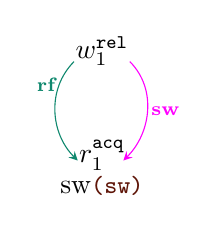
\begin{tikzpicture}[x=1em,y=1em,yscale=-1,xscale=-1]
\tikzstyle{every node}=[font=\normalfont]
\node (w1) {$ w^\rel_1 $};
\node (r1) [below=20pt of w1] {$ r^\acq_1 $};
\node (sw) [below=-5pt of r1] {\hlref{sw}};

\draw [->,>=stealth,color=Magenta] ($ (w1.south east)+(.3,-5pt) $) to[out=135,in=-135] node[midway,right=-2pt,font=\scriptsize] {\textcolor{black}{\lsw}} ($ (r1.south east)+(0.4,-7pt) $);
\draw [->,>=stealth,color=PineGreen] ($ (w1.south west)+(-.3,-5pt) $) to[out=45,in=-45] node[left=-2pt,pos=.25,font=\scriptsize] {\textcolor{black}{\lrf}}($ (r1.south west)+(-0.3,-7pt) $);

\end{tikzpicture}
} &
		\resizebox{0.14\textwidth}{!}{\tikzset{every picture/.style={line width=0.75pt}} %set default line width to 0.75pt        
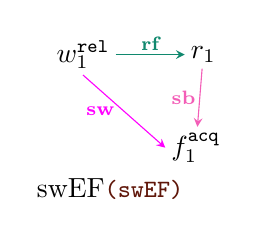
\begin{tikzpicture}[x=1em,y=1em,yscale=-1,xscale=-1]
\tikzstyle{every node}=[font=\normalfont]
\node (w1) [inner sep=2pt] {$ w^\rel_1 $};
\node (r1) [right=25pt of w1,inner sep=2pt] {$ r_1 $};
\node (f1) [below left=21pt and -15pt of r1,inner sep=2pt] {$ f^\acq_1 $};
\node (swef) [below left=0pt and -10pt of f1] {\hlref{swEF}};

`\draw [->,>=stealth,color=Magenta,thin] (w1.south) -- node[midway,left=0pt,font=\scriptsize,color=black] { $\lsw$ } (f1.west);
\draw [->,>=stealth,color=PineGreen,thin] (w1) -- node[midway,above=-2pt,font=\scriptsize,color=black] { $ \lrf $ }  (r1);
\draw [->,>=stealth,color=CarnationPink,thin] (r1) -- node[midway,left=-2pt,font=\scriptsize,color=black] { $\lsb$ } (f1);

\end{tikzpicture}
} &
		\resizebox{0.14\textwidth}{!}{\tikzset{every picture/.style={line width=0.75pt}} %set default line width to 0.75pt        
\begin{tikzpicture}[x=1em,y=1em,yscale=-1,xscale=-1]
\tikzstyle{every node}=[font=\normalfont]
\node [inner sep=2pt] (f1) {$ f^\rel_1 $};
\node (w1) [below left=21pt and -15pt of f1,inner sep=2pt] {$ w_1 $};
\node (r1) [right=25pt of w1,inner sep=2pt] {$ r^\acq_1 $};
\node (swfe) [below right=0pt and -15pt of wr1] {\hlref{sw-dobFE}};

`\draw [->,>=stealth,color=Magenta,thin] (f1.east) -- node[midway,right=0pt,font=\scriptsize,color=black] { $\lsw$ } (r1.north);
\draw [->,>=stealth,color=PineGreen,thin] (w1) -- node[midway,above=-2pt,font=\scriptsize,color=black] { $ \lrf $ } (r1);
\draw [->,>=stealth,color=CarnationPink,thin] (f1) -- node[midway,left=-2pt,font=\scriptsize,color=black] { $\lsb$ } (w1);

\end{tikzpicture}
} &
		\resizebox{0.17\textwidth}{!}{\tikzset{every picture/.style={line width=0.75pt}} %set default line width to 0.75pt        
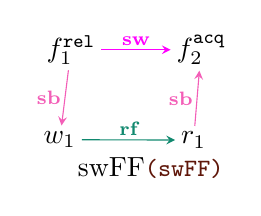
\begin{tikzpicture}[x=1em,y=1em,yscale=-1,xscale=-1]
\tikzstyle{every node}=[font=\normalfont]
\node (f1) [inner sep=2pt] {$ f^\rel_1 $};
\node (f2) [right=25pt of f1,inner sep=2pt] {$ f^\acq_2 $};
\node (w1) [below left=20pt and -15pt of f1,inner sep=2pt] {$ w_1 $};
\node (r1) [below left=20pt and -15pt of f2,inner sep=2pt] {$ r_1 $};
\node (swff) [below right=-2pt and -5pt of w1] {\hlref{swFF}};

`\draw [->,>=stealth,color=Magenta] (f1) -- node[midway,above=-2pt,font=\scriptsize,color=black] { $\lsw$ } (f2);
\draw [->,>=stealth,color=PineGreen] (w1) -- node[midway,above=-2pt,font=\scriptsize,color=black]{\lrf} (r1);
\draw [->,>=stealth,color=CarnationPink] (f1) -- node[midway,left=-2pt,font=\scriptsize,color=black] { $\lsb$ } (w1);
\draw [->,>=stealth,color=CarnationPink] (r1) -- node[midway,left=-2pt,font=\scriptsize,color=black] { $\lsb$ } (f2);

%\draw [->,>=stealth,color=orange] ($ (ew1.south east)+(.5,-5pt) $) to[out=135,in=-135] node[midway,right=-2pt,font=\scriptsize] {mo} ($ (ew2.south east)+(0.4,-5pt) $);
%\draw [->,>=stealth,color=red] ($ (ew1.south west)+(-.3,-5pt) $) to[out=45,in=-45] node[midway,left=-2pt,font=\scriptsize] {c::hb} ($ (ew2.south west)+(-0.3,-5pt) $);


\end{tikzpicture}
} &
		
		\resizebox{0.16\textwidth}{!}{\tikzset{every picture/.style={line width=0.75pt}} %set default line width to 0.75pt        
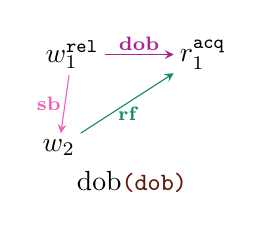
\begin{tikzpicture}[x=1em,y=1em,yscale=-1,xscale=-1]
\tikzstyle{every node}=[font=\normalfont]
\node (w1) [inner sep=2pt] {$ w^\rel_1 $};
\node (r1) [right=25pt of w1,inner sep=2pt] {$ r^\acq_1 $};
\node (w2) [below left=21pt and -15pt of w1,inner sep=2pt] {$ w_2 $};
\node (dob) [below right=0pt and -5pt of w2] {\hlref{dob}};

`\draw [->,>=stealth,color=Mulberry] (w1.east) -- node[midway,above=-2pt,font=\scriptsize,color=black] { $\ldob$ } (r1.west);
\draw [->,>=stealth,color=PineGreen] (w2) -- node[midway,below=-2pt,font=\scriptsize,color=black] { $ \lrf $ }  (r1);
\draw [->,>=stealth,color=CarnationPink] (w1) -- node[midway,left=-2pt,font=\scriptsize,color=black] { $\lsb$ } (w2);

\end{tikzpicture}
} &
		\resizebox{0.17\textwidth}{!}{\tikzset{every picture/.style={line width=0.75pt}} %set default line width to 0.75pt        
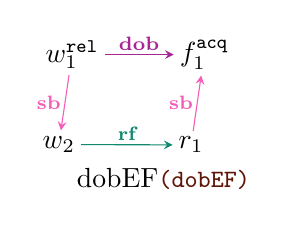
\begin{tikzpicture}[x=1em,y=1em,yscale=-1,xscale=-1]
\tikzstyle{every node}=[font=\normalfont]
\node (w1) [inner sep=2pt] {$ w^\rel_1 $};
\node (f1) [right=25pt of w1,inner sep=2pt] {$ f^\acq_1 $};
\node (w2) [below left=20pt and -15pt of w1,inner sep=2pt] {$ w_2 $};
\node (r1) [below left=20pt and -13pt of f1,inner sep=2pt] {$ r_1 $};
\node (dobEF) [below right=0pt and -5pt of w2] {\hlref{dobEF}};

`\draw [->,>=stealth,color=PineGreen,thin] (w2) -- node[midway,above=-2pt,font=\scriptsize,color=black] { $\lrf$ } (r1);
\draw [->,>=stealth,color=CarnationPink,thin] (w1) -- node[midway,left=-2pt,font=\scriptsize,color=black] { $ \lsb $ } (w2);
\draw [->,>=stealth,color=CarnationPink,thin] (r1) -- node[midway,left=-2pt,font=\scriptsize,color=black] { $\lsb$ } (f1);
\draw [->,>=stealth,color=Mulberry,thin] (w1) -- node[midway,above=-2pt,font=\scriptsize,color=black] { $\ldob$ } (f1);

\end{tikzpicture}
} \\
		\hline
		\multicolumn{4}{c}{(a) \lsw relation} &
		\multicolumn{2}{c}{(b) \ldob relation} \\
	\end{tabular}
	\label{fig:sw}
\end{figure}

\noindent
Formally, $\setSW$ relation is formed using fences as,

$\forall e_1, e_2 \in \events_\tau$ \st $\rf{\tau}{e_1}{e_2}$

if
$e_1 \in \ordwrites{\moge\rel}_\tau$, 
$\exists \mathbb{F}^\acq \in \ordfences{\moge\acq}_{\tau}$ where
$\seqb{\tau}{e_2}{\mathbb{F}^\acq}$ then
$\sw{\tau}{e_1}{\mathbb{F}^\acq}$;

if
$e_2 \in \ordreads{\moge\acq}_\tau$, 
$\exists \mathbb{F}^\rel \in \ordfences{\moge\rel}_{\tau}$ where
$\seqb{\tau}{\mathbb{F}^\rel}{e_1}$ then
$\sw{\tau}{\mathbb{F}^\rel}{e_2}$;

if
$\exists \mathbb{F}^\rel \in \ordfences{\moge\rel}_{\tau}$,
$\mathbb{F}^\acq \in \ordfences{\moge\acq}_{\tau}$ where
$\seqb{\tau}{\mathbb{F}^\rel}{e_1}$,
$\seqb{\tau}{e_2}{\mathbb{F}^\acq}$ 

then
$\sw{\tau}{\mathbb{F}^\rel}{\mathbb{F}^\acq}$.

\noindent
Similarly, $\setDOB$ relation is formed using fences as,

$\forall e_1, e_2 \in \events_\tau$, 
$e_1' \in \ordwrites{\moge\rel}_\tau$ \st $\rf{\tau}{e_1}{e_2}$
and $e_1 \in$ {\em release-sequence}($e_1'$)

if $\exists \mathbb{F}^\acq \in \ordfences{\moge\acq}_{\tau}$ 
where $\seqb{\tau}{e_2}{\mathbb{F}^\acq}$ then
$\dob{\tau}{e_1'}{\mathbb{F}^\acq}$.

\noindent
Further, as is the case with program events,
if $\sw{\tau}{e_1}{e_2}$ or $\dob{\tau}{e_1}{e_2}$ then
events $e_1',e_2'$ \st $\seqb{\tau}{e_1'}{e_1}$ and 
$\seqb{\tau}{e_2}{e_2'}$ are related as $\ithb{\tau}{e_1'}{e_2'}$.

\section{title for sc theory} \label{sec:theory}
\section{Methodology} \label{sec:methodology}
\section{Implementation Details} \label{sec:implementation}
\section{Results} \label{sec:results}
\section{Related Work} \label{sec:related}
\section{Conclusion} \label{sec:conclusion}

%\bibliographystyle{unsrtnat}
\bibliography{References.bib}


\end{document}
